\section{Results}
\subsection{Physics-based estimators}
Table~\ref{tab:socphys} and Fig.~\ref{fig:traj} show that the EKF stays below 1.1 points MAE on all three unseen conditions, including the 1\,A test, and removes a 30-point initial error within the excluded 10\,min warm-up, whereas Coulomb counting drifts linearly because $Q_{\mathrm{cal}}$ differs from the capacity actually delivered (3.2--6.4 points) and keeps a wrong initial SOC. Identifying parameters on the same test lowers the EKF MAE to about 0.12 points (in-sample, optimistic; see \texttt{docs/EXPERIMENTAL\_RESULTS.md}).
\begin{table}[htbp]\centering\footnotesize
\begin{tabular}{llrrrr}
\toprule
 &  & MAE & RMSE & R$^2$ & MaxAE \\
Test & Estimator &  &  &  &  \\
\midrule
\multirow[t]{4}{*}{0\,°C} & CC (SOC$_0$=100\%) & 6.44 & 7.40 & 0.93 & 12.76 \\
 & EKF (SOC$_0$=100\%) & 0.71 & 0.86 & 1.00 & 2.74 \\
 & CC (SOC$_0$=70\%) & 23.56 & 23.85 & 0.31 & 29.89 \\
 & EKF (SOC$_0$=70\%) & 0.71 & 0.86 & 1.00 & 2.74 \\
\cline{1-6}
\multirow[t]{4}{*}{45\,°C} & CC (SOC$_0$=100\%) & 3.15 & 3.62 & 0.98 & 6.24 \\
 & EKF (SOC$_0$=100\%) & 1.02 & 1.13 & 1.00 & 2.22 \\
 & CC (SOC$_0$=70\%) & 26.85 & 26.91 & 0.12 & 29.94 \\
 & EKF (SOC$_0$=70\%) & 1.03 & 1.14 & 1.00 & 2.22 \\
\cline{1-6}
\multirow[t]{4}{*}{1\,A} & CC (SOC$_0$=100\%) & 3.69 & 4.12 & 0.98 & 6.84 \\
 & EKF (SOC$_0$=100\%) & 0.66 & 0.75 & 1.00 & 1.40 \\
 & CC (SOC$_0$=70\%) & 26.31 & 26.37 & 0.02 & 29.45 \\
 & EKF (SOC$_0$=70\%) & 0.69 & 0.77 & 1.00 & 1.38 \\
\cline{1-6}
\bottomrule
\end{tabular}
\caption{Physics-based SOC estimators (capacity and ECM calibrated on the 25\,°C test) on unseen conditions; errors in SOC points, first 10\,min excluded.}\label{tab:socphys}
\end{table}

\begin{figure}[H]\centering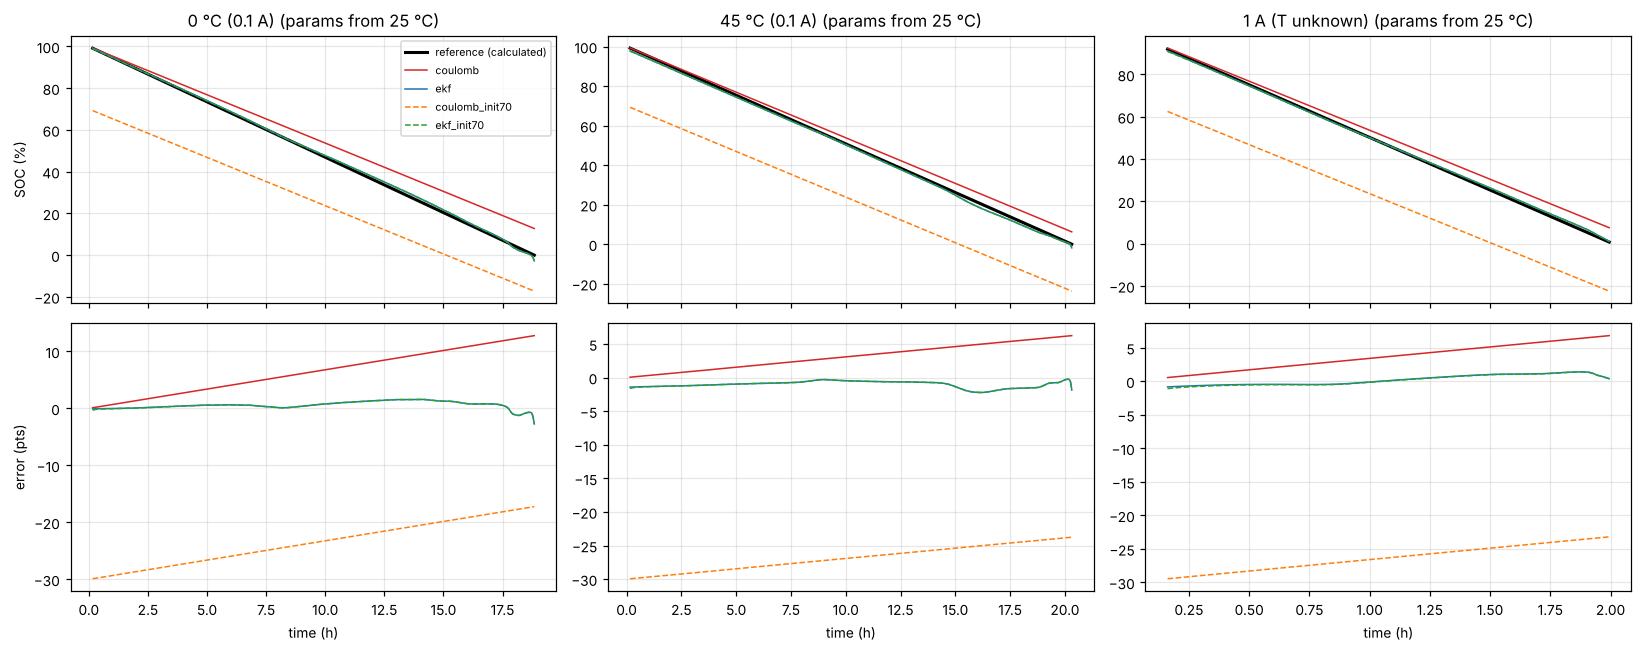
\includegraphics[width=\linewidth]{fig03_physics_soc_trajectories.png}\caption{SOC trajectories and errors of CC and EKF (parameters from 25\,°C) with correct and wrong (70\,\%) initial SOC.}\label{fig:traj}\end{figure}

\subsection{Data-driven estimators and comparative analysis}
Table~\ref{tab:socdd} and Fig.~\ref{fig:dd} give the cross-condition errors. Random Forest and gradient boosting reach 0.4--1.6 points on the 0.1\,A cross-temperature cases and fail on the 1\,A test (13--14 points), because the current lies far outside the training range and the voltage sag is read as lower SOC. The NumPy LSTM/GRU are less accurate and more variable (GRU in particular); their hyper-parameters were not optimised, so no general conclusion on recurrent models is drawn.
\begin{table}[htbp]\centering\footnotesize
\begin{tabular}{lrrrrrr}
\toprule
 & random\_forest & hist\_gradient\_boosting & gru & gru\_sf & lstm & lstm\_sf \\
Train $\rightarrow$ Test &  &  &  &  &  &  \\
\midrule
0\,°C+25\,°C $\rightarrow$ 45\,°C & 1.53 & 1.55 & 9.84 & 6.85 & 1.78 & 1.67 \\
0\,°C+25\,°C+45\,°C $\rightarrow$ 1\,A & 13.20 & 12.96 & 53.46 & 37.63 & 53.01 & 24.37 \\
0\,°C+45\,°C $\rightarrow$ 25\,°C & 1.41 & 1.53 & 11.33 & 9.47 & 1.24 & 1.06 \\
25\,°C $\rightarrow$ 0\,°C & 0.43 & 0.42 & 5.88 & 6.36 & 4.97 & 2.39 \\
25\,°C $\rightarrow$ 1\,A & 13.06 & 14.40 & 29.01 & 101.99 & 42.95 & 41.12 \\
25\,°C $\rightarrow$ 45\,°C & 1.57 & 1.56 & 6.19 & 5.37 & 3.97 & 2.05 \\
25\,°C+45\,°C $\rightarrow$ 0\,°C & 0.75 & 0.69 & 7.06 & 7.51 & 0.92 & 1.04 \\
\bottomrule
\end{tabular}
\caption{Data-driven SOC models: MAE (SOC points) on the unseen test condition (clean signals). \texttt{*\_sf}: std-floor scaling variant added post hoc.}\label{tab:socdd}
\end{table}

\begin{figure}[H]\centering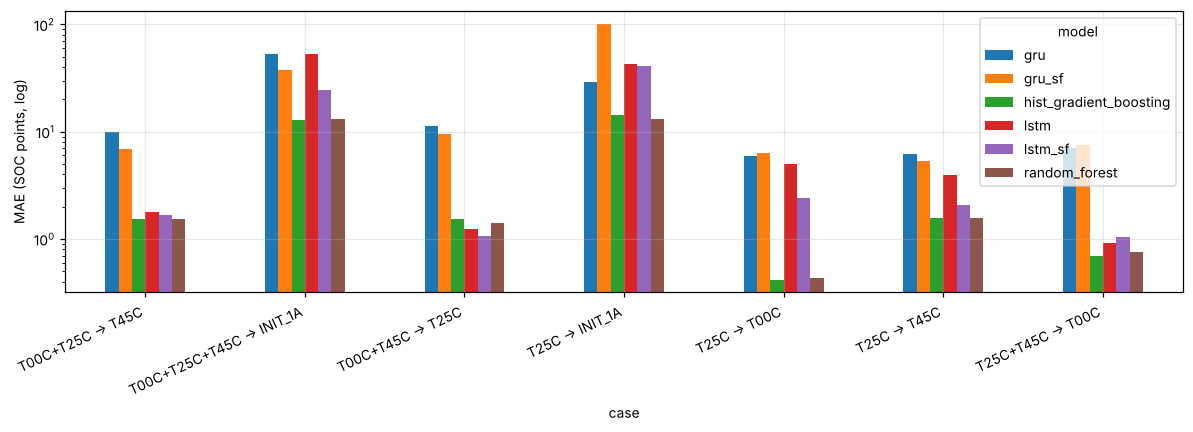
\includegraphics[width=0.85\linewidth]{fig05_data_driven_protocols.png}\caption{MAE of data-driven models per protocol (log scale).}\label{fig:dd}\end{figure}

\subsection{Temperature influence}
Measured delivered capacity at 0.1\,A is 1.882\,Ah at 0\,°C (87\,\% of the 25\,°C value) and $R_0$ at discharge onset is 0.132\,$\Omega$ versus 0.080\,$\Omega$ at 25\,°C (Fig.~\ref{fig:cap}). The EKF and CC, which carry a fixed calibrated capacity, show the corresponding error (CC 6.4 points at 0\,°C). In contrast, data-driven models score well across temperature, but this is largely because each test's reference is normalised by its own capacity, so the capacity change is invisible to the target; the result must not be read as robustness to real capacity variation. Voltage versus reference SOC is nearly temperature-independent at 0.1\,A (Fig.~\ref{fig:vsoc}).
\begin{figure}[H]\centering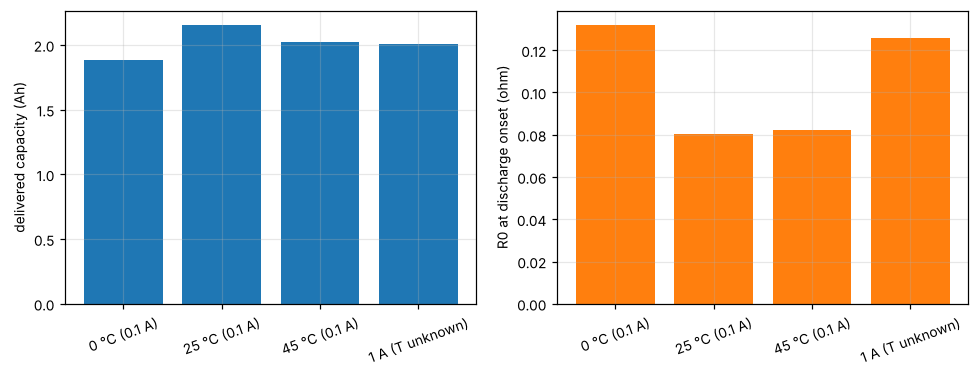
\includegraphics[width=\linewidth]{fig07_capacity_and_r0.png}\caption{Delivered capacity and $R_0$ per condition (labels, not measured temperatures).}\label{fig:cap}\end{figure}
\begin{figure}[H]\centering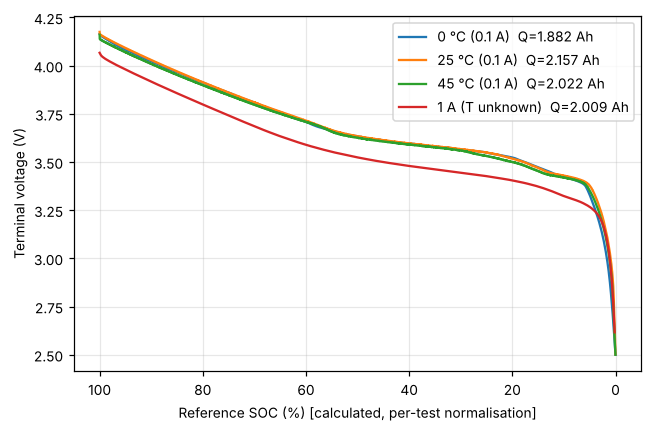
\includegraphics[width=0.6\linewidth]{fig02_voltage_vs_soc_ref.png}\caption{Voltage versus calculated reference SOC.}\label{fig:vsoc}\end{figure}

\subsection{Noise robustness and computational cost}
Table~\ref{tab:noise} (Fig.~\ref{fig:noise}): the EKF is insensitive to noise at its fixed covariance (0.9 points mean MAE), but a 20\,mA current bias raises Coulomb counting to 14 points. Trees degrade gently; the original LSTM/GRU collapse (tens of points) because standardising a nearly constant current (standard deviation of only 0.1--1.6\,mA on the 20\,s grid in the three low-current tests) amplifies noise, which the \texttt{*\_sf} variants remove. Inference costs are in Table~\ref{tab:timing}; all are far below real-time limits at 20\,s sampling.
\begin{table}[htbp]\centering\footnotesize
\begin{tabular}{lrrrrr}
\toprule
 & clean & low & medium & high & I bias 20\,mA \\
\midrule
coulomb & 4.79 & 4.78 & 4.77 & 4.75 & 13.95 \\
ekf & 0.87 & 0.86 & 0.86 & 0.85 & 1.19 \\
random\_forest & 1.00 & 1.01 & 1.05 & 1.16 & 1.00 \\
hist\_gradient\_boosting & 0.99 & 1.05 & 1.20 & 1.66 & 0.98 \\
gru & 6.03 & 60.64 & 70.63 & 70.64 & 25.35 \\
gru\_sf & 5.87 & 5.91 & 6.26 & 7.43 & 8.48 \\
lstm & 4.47 & 18.99 & 22.34 & 28.15 & 24.89 \\
lstm\_sf & 2.22 & 2.27 & 2.41 & 2.89 & 3.43 \\
\bottomrule
\end{tabular}
\caption{Noise robustness with \emph{simulated} perturbations (Table~\ref{tab:noisedef}) added to the real test signals: mean MAE (SOC points) over the 0\,°C and 45\,°C tests, models fitted on 25\,°C.}\label{tab:noise}
\end{table}

\begin{figure}[H]\centering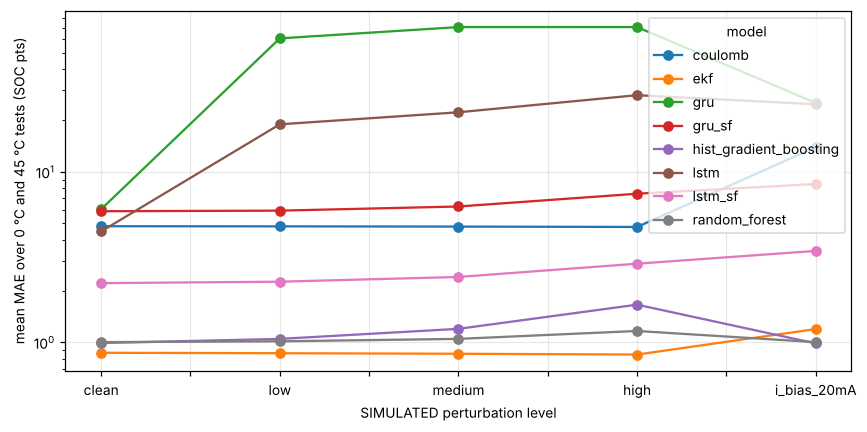
\includegraphics[width=0.75\linewidth]{fig06_noise_robustness.png}\caption{Noise robustness (simulated perturbations).}\label{fig:noise}\end{figure}
\begin{table}[htbp]\centering\footnotesize
\begin{tabular}{lr}
\toprule
 & ms per 1000 samples \\
\midrule
coulomb & 0.02 \\
coulomb\_init70 & 0.02 \\
ekf & 46.93 \\
ekf\_init70 & 46.96 \\
ekf\_matched & 48.33 \\
gru & 14.53 \\
gru\_sf & 14.13 \\
hist\_gradient\_boosting & 4.48 \\
lstm & 21.42 \\
lstm\_sf & 21.32 \\
random\_forest & 11.54 \\
\bottomrule
\end{tabular}
\caption{Mean inference time (NumPy/scikit-learn/Python, single CPU core). The EKF figure is a plain Python loop.}\label{tab:timing}
\end{table}


\subsection{SOH and RUL}
SOH(\%) is not computed: nominal capacity is unverified and one cycle per file gives no degradation trajectory. RUL is not defined for the same reasons (\texttt{results/experiment\_logs/soh\_rul\_feasibility.json}). The delivered-capacity ratios of Table~\ref{tab:capacity} mix temperature, rate and history and are not SOH.

\subsection{Fault diagnosis}
On real data the detectors flag few windows (Table~\ref{tab:faultreal}); of the 80 top-ranked windows (20 per dataset), 50 lie within two minutes of a protocol step transition and are labelled as probable operational events by the decision layer; the remaining 30 are unexplained statistical anomalies. None constitutes evidence of a real fault. The persistence rule fires on constant-voltage charge phases, which are expected. On \emph{simulated} faults (Tables~\ref{tab:faultsim10}, \ref{tab:faultsim05}) the combined detector finds every event at magnitude $\times$1 and $\times$0.5, with different detectors responsible for different fault types; at magnitude $\times$0.25 the extra-resistance fault is missed. Window precision of the combined detector is low (0.24--0.55 at $\times$1), because detectors also flag genuine transitions.
\begin{table}[htbp]\centering\footnotesize
\begin{tabular}{lrrrrrr}
\toprule
 & windows & IF & OC-SVM & Thr. & Flat. & Any \\
\midrule
0\,°C & 5239 & 33 & 37 & 45 & 37 & 96 \\
25\,°C & 5646 & 31 & 33 & 10 & 0 & 39 \\
45\,°C & 5511 & 21 & 17 & 9 & 0 & 25 \\
1\,A & 1116 & 20 & 221 & 44 & 75 & 245 \\
\bottomrule
\end{tabular}
\caption{Windows flagged on the \emph{real} data (statistical anomalies, not validated faults); detectors fitted on 0\,°C and 45\,°C windows.}\label{tab:faultreal}
\end{table}

\begin{table}[htbp]\centering\footnotesize
\begin{tabular}{lrrrrr}
\toprule
 & IF & OC-SVM & Threshold & Flatline & Any \\
\midrule
current\_sensor\_offset & 1.00 & 1.00 & 1.00 & 0.00 & 1.00 \\
resistance\_increase & 1.00 & 1.00 & 0.00 & 0.00 & 1.00 \\
sample\_dropout & 0.25 & 1.00 & 0.00 & 0.00 & 1.00 \\
voltage\_sensor\_stuck & 0.00 & 0.00 & 0.00 & 1.00 & 1.00 \\
voltage\_spike & 1.00 & 1.00 & 1.00 & 0.00 & 1.00 \\
\bottomrule
\end{tabular}
\caption{\emph{Simulated} faults (magnitude $\times$1.0) injected into the real 25\,°C signals: event detection rate (4 events per fault type).}\label{tab:faultsim10}
\end{table}

\begin{table}[htbp]\centering\footnotesize
\begin{tabular}{lrrrrr}
\toprule
 & IF & OC-SVM & Threshold & Flatline & Any \\
\midrule
current\_sensor\_offset & 1.00 & 1.00 & 1.00 & 0.00 & 1.00 \\
resistance\_increase & 1.00 & 0.00 & 0.00 & 0.00 & 1.00 \\
sample\_dropout & 0.25 & 1.00 & 0.00 & 0.00 & 1.00 \\
voltage\_sensor\_stuck & 0.00 & 0.00 & 0.00 & 1.00 & 1.00 \\
voltage\_spike & 1.00 & 1.00 & 0.00 & 0.00 & 1.00 \\
\bottomrule
\end{tabular}
\caption{\emph{Simulated} faults (magnitude $\times$0.5) injected into the real 25\,°C signals: event detection rate (4 events per fault type).}\label{tab:faultsim05}
\end{table}

\begin{figure}[H]\centering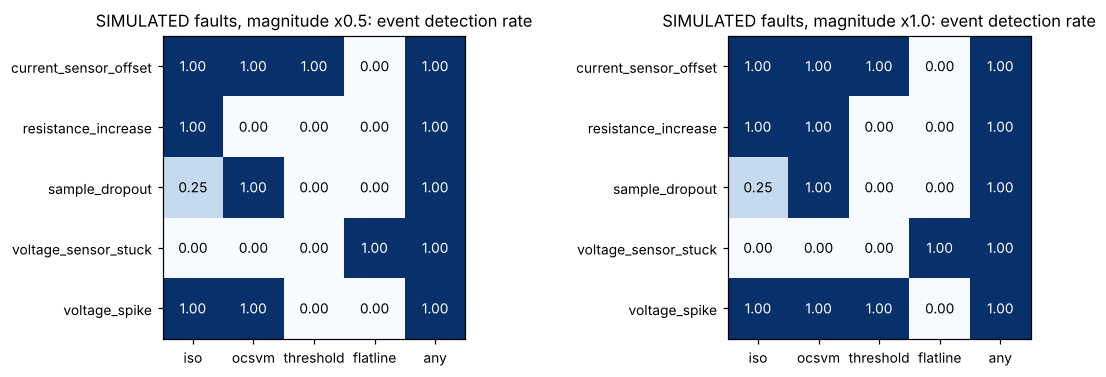
\includegraphics[width=\linewidth]{fig08_fault_simulation_detection.png}\caption{Event detection on \emph{simulated} faults.}\end{figure}

\subsection{Discussion}
The EKF is the most reliable estimator across temperature and rate in this study because its physical structure handles the voltage drop and corrects initial errors; tree models are accurate only inside the training regime; recurrent networks need more data and tuning. All conclusions hold for one cell and constant-current tests.
